% #######################################
% ########### FILL THESE IN #############
% #######################################
\def\mytitle{Coursework Report}
\def\myauthor{Maria Luque Anguita}
\def\contact{40280156@napier.ac.uk}
\def\mymodule{Web Technologies (SET08101)}
% #######################################
% #### YOU DON'T NEED TO TOUCH BELOW ####
% #######################################
\documentclass[10pt, a4paper]{article}
\usepackage[a4paper,outer=1.5cm,inner=1.5cm,top=1.75cm,bottom=1.5cm]{geometry}
\twocolumn
\usepackage{graphicx}
\graphicspath{{./images/}}
%colour our links, remove weird boxes
\usepackage[colorlinks,linkcolor={black},citecolor={blue!80!black},urlcolor={blue!80!black}]{hyperref}
%Stop indentation on new paragraphs
\usepackage[parfill]{parskip}
%% Arial-like font
\usepackage{lmodern}
\renewcommand*\familydefault{\sfdefault}
%Napier logo top right
\usepackage{watermark}
%Lorem Ipusm dolor please don't leave any in you final report ;)
\usepackage{lipsum}
\usepackage{xcolor}
\usepackage{listings}
%give us the Capital H that we all know and love
\usepackage{float}
%tone down the line spacing after section titles
\usepackage{titlesec}
%Cool maths printing
\usepackage{amsmath}
%PseudoCode
\usepackage{algorithm2e}

\titlespacing{\subsection}{0pt}{\parskip}{-3pt}
\titlespacing{\subsubsection}{0pt}{\parskip}{-\parskip}
\titlespacing{\paragraph}{0pt}{\parskip}{\parskip}
\newcommand{\figuremacro}[5]{
    \begin{figure}[#1]
        \centering
        \includegraphics[width=#5\columnwidth]{#2}
        \caption[#3]{\textbf{#3}#4}
        \label{fig:#2}
    \end{figure}
}

\lstset{
	escapeinside={/*@}{@*/}, language=C++,
	basicstyle=\fontsize{8.5}{12}\selectfont,
	numbers=left,numbersep=2pt,xleftmargin=2pt,frame=tb,
    columns=fullflexible,showstringspaces=false,tabsize=4,
    keepspaces=true,showtabs=false,showspaces=false,
    backgroundcolor=\color{white}, morekeywords={inline,public,
    class,private,protected,struct},captionpos=t,lineskip=-0.4em,
	aboveskip=10pt, extendedchars=true, breaklines=true,
	prebreak = \raisebox{0ex}[0ex][0ex]{\ensuremath{\hookleftarrow}},
	keywordstyle=\color[rgb]{0,0,1},
	commentstyle=\color[rgb]{0.133,0.545,0.133},
	stringstyle=\color[rgb]{0.627,0.126,0.941}
}

\thiswatermark{\centering \put(336.5,-38.0){
\includegraphics[scale=0.8]{logo}} }
\title{\mytitle}
\author{\myauthor\hspace{1em}\\\contact\\Edinburgh Napier University\hspace{0.5em}-\hspace{0.5em}\mymodule}
\date{}
\hypersetup{pdfauthor=\myauthor,pdftitle=\mytitle,pdfkeywords=\mykeywords}
\sloppy
% #######################################
% ########### START FROM HERE ###########
% #######################################
\begin{document}
	\maketitle
	\begin{abstract}
	    In this coursework the aim is to design and code a blog journal. A blog is an informational website where the owner or owners of the blog share their views on a subject. The posts might be all related, for example if the blog is a fashion blog, the posts will all have different outfits, or makeup tutorials, etc... Or each post might be of a different topic. The website displays the posts in order, with the latest post at the top, so viewers keep up to date with it.
	\end{abstract}


	\section{Introduction}
	My blog is called "Maria Around the World Blog" and the name is clearly displayed at the top in the header image. It is a personal blog dedicated to my travel experiences, fashion and other topics of which I am passionate about.

	The pages that the user can go to are:

	\begin{itemize}
        \item Blog: a page where all the posts are displayed chronologically
        \item About me: this page displays basic information about me like where I come from, what I currently study and my hobbies
        \item Work with me: displays email and phone number for collaboration requests
    \end{itemize}

    Every viewer can go to the 'About me' and 'Work with me' pages but if they want to see the blog or post something they will have to register and login.

    At the bottom of each page there are two sections, one includes my social media with images of them that if clicked, takes the user to the respective profile; and the other section is where users will be able to subscribe. It also displays the number of monthly subscribers at the bottom, which is a very motivating part of the blog.

    To program this blog I did some background reading. To start understanding what the code had to look like I skimmed over the book 'Beginning Node.js' [1] and used an online learning center 'Stackskills' [2] to practice using Node.js. I also watched some video tutorials from YouTube [3] to get me started.

    \section{Software Design}

    The first thing I did was look at various fashion blogs [4] and sketch a typical blog in a piece of paper so I could have an idea of what mine should include and how it would look like:

    \includegraphics[width=8cm]{sketch.jpg}

    \textbf{Figure 1 Brief sketch}
    \vspace{2mm}

    This was the first sketch, which only included a main post as you open the page and the social media links.The aim was to have a navigation bar to allow the user to easily travel between the different pages within the site, the picture above demonstrates this. From the outline, each post would contain a title and text box for the actual content of the post, while a footer along the bottom would display the latest additions to the platform.


    This idea was inspired from the blog 'The Blonde Salad', which is owned by the most known blogger globally, Chiara Ferragni.

    The idea was to only let the user post, edit, and delete posts, while if the user is not logged in, it will only be able to access 'About me' and 'Work with me', along with the options to Register or Login:

    \includegraphics[width=8cm]{views1.jpg}
    \includegraphics[width=8cm]{views2.jpg}
    \textbf{Figure 2 Navigation diagram}
    \vspace{2mm}

    Since the beginning I had a list of requirements that I wanted to include. Which was:
    \begin{itemize}
        \item Rewarding user experience: nice colours (probably pastels), easy to navigate through it
        \item Pictures, a lot of them
        \item Post displayed in reverse order, in chronological order
        \item Social media links
        \item Somewhere to subscribe
        \item Allow comments from viewers
        \item How to contact me
    \end{itemize}

    Many of these ideas came from a webpage that highlighted the features a successful blog must have [5].
    Once I had all of this, I was ready to start coding.




    \section{Implementation}
    For this coursework, I use Node.js to write JavaScript code for the server side.

    For the client interface, all relevant .jade files where used instead of HTML because Jade is much more error-proof, given that you don't need to use closing tags and it looks cleaner [7]. They are in the views folder of the project. These allow me to design my site.

    In order to connect the client and server elements, the use of Mongoose (an object modeling package for Node) was required. This acted as a bridge between MongoDB, the database and Node.js and provided a create, read, update, delete (CRUD) API that the client element uses to provide the blog's features. Mongoose allowed me to have access to the MongoDB commands for CRUD simply and easily. Once I installed the mongoose package and added it to my project, all I had to do was connect to my local database and create a Schema [6] to save objects.

    When the viewer opens the webpage, the first thing to see will be the Login page, but from there it can access other parts of the website too apart from the Blog if the user is not logged in:

    \includegraphics[width=8cm]{login1.jpg}

    \textbf{Figure 3 Login page}
    \vspace{2mm}

    After every single page there are another two block at the bottom of the page where the social media links and subscribers part are, therefore they can be accessible from anywhere:

    \includegraphics[width=8cm]{followme.jpg}

    \textbf{Figure 4 Blocks at the bottom of the page}
    \vspace{2mm}

    For this website, the main color is a dark pink, very pastel. The inspiration to use this color came from a very well organised blog [8] which uses this colour in its logo.
    The background is not white, it is instead a very light grey that makes the web page less shiny and therefore easier to be looking at it.

    The airplane on the side suits the blog perfectly because as the title suggests, Maria is around the world, therefore getting in a lot of planes. It is a simple airplane leaving a trace behind it that decorates the sides of the web page. However, as the web page is made thinner, for example into mobile form, the airplane and the trace at both sides disappear so the user can view the blog more comfortably. They were done using Canva [11].
    All different parts of the web page have a pink rounded border to divide the blog clearly. Links to social media are located and also provide a colourful view alongside with an image of me so users know exactly who the main owner of the blog is.

    In the navigation bar, there is a section called 'Work with me' which is accessible at any time and contains images and information to contact me like email and phone number.

    \includegraphics[width=7cm]{work.jpg}

    \textbf{Figure 5 Work with me section}
    \vspace{2mm}

    Similar to this page is the page 'About me' which is also made up of images with information about me.

    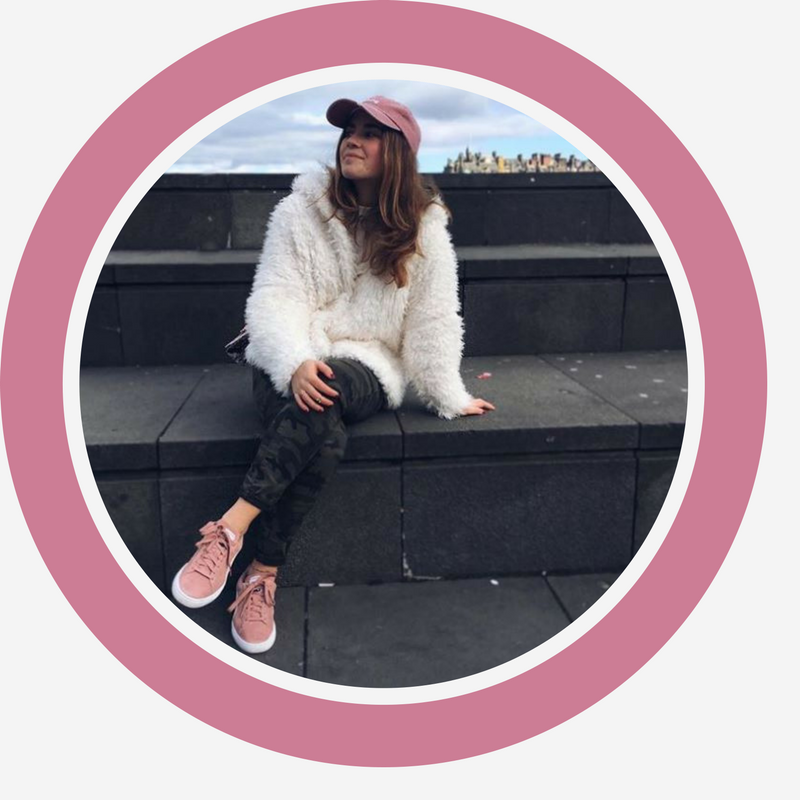
\includegraphics[width=7cm]{aboutme.jpg}

    \textbf{Figure 6 About me section}
    \vspace{2mm}

    Once the person is logged in or registered, those options disappear from the navigation bar and 'Log out' appears as an option.
    They also have access to the Blog part now that they are logged in. This part contains the posts in chronological order, last one posted first.

    All of the posts follow the same layout: Post title, category it was posted in along with date and name of author, post image, a bit of truncated text from the original post and three options, Read more, Edit or Delete.

    \includegraphics[width=8cm]{post.jpg}

    \textbf{Figure 7 Example of post in blog feed}
    \vspace{2mm}

    I also added a commenting feature in each individual post, since I believe this is one of the most important features of a blog, where people express their opinion about the matter discussed.
    All of the comments are pushed to the database in each specific post they are. Therefore a single post might have various comments.

    \includegraphics[width=8cm]{comment.jpg}

    \textbf{Figure 8 Commenting feature}
    \vspace{2mm}

    To add security to the blog, when users first register, their password is encrypted using 'bcrypt' [9]. The bcrypt package website provides an overview of how to hash a password, which was then implemented in my project:

    \begin{lstlisting}[caption = How to hash a password]
bcrypt.genSalt(saltRounds, function(err, salt) {
    bcrypt.hash(myPlaintextPassword, salt, function(err, hash) {
        // Store hash in your password DB.
    });
});
    \end{lstlisting}

    Then all that was left to do was update that code to suit my project and make it look nice using CSS. There is a single CSS file for the whole blog.




    \section{Critical Evaluation}

    \subsection{Comparison against requirements}

The requirements for this assignment are to design and implement a simple blog platform with server and client elements. This blog presents a user interface enabling users to add new blog posts, edit, view and delete existing posts. The server persists data and provides a CRUD API that the client can use.

It also has more advanced features that have not been specifically covered in the practical sessions and which I  have investigated for myself, like managing users. Another requirement was to evaluate the design using appropriate techniques.

A blog can be evaluated asking a few simple questions [10]. The first one is why. What is the purpose of the blog, which is to share peoples views on previous experiences travelling around the world.

First impressions are very important since they can be nearly impossible to reverse or undo. If the person doesn't think it is going to be easy to navigate through the blog, they will just not use it. This goes along with usability, this blog has separate sections for different parts and all are labelled clearly in a clear font. It should also have a good graphical presentation and be 'pleasing to the eye'.

    \subsection{Comparison against other blog platforms }
Most blog platforms are similar to my blog, except with more features, but those are improvements that could always be done to my blog.

Most of the blogs available are only coded so that there is a single administrator changing it. However in my blog, everyone registered can post in it, which I think is better.

    \subsection{Possible improvements}

There  is  always  room  for  improvement,  even  if  the  blog meets  its  requirements,  updates  can  always  make  it  better.In this case, I feel some features could be added to different parts of the website.

Regarding  CSS  (the  design  of  the  website),  the  homepage could be altered by giving it a different touch, instead of making  the  typical  blog  homepage. In the near future, I will update the look of blog and add a grid where there is a photo for each section of the blog and it looks like a collage occupying the whole page instead of having a navigation bar at the top.

It should also include a search engine, to look for posts or a list of all the posts in the side. I will also include replies and likes to comments and an Instagram plugin.



    \section{Personal Evaluation}

Because of this coursework I have learned what client and server sides includes, how they work... I also learned about the existence of Node.js and Jade files, since I had not heard about them before. It also broadened my knowledge of CSS since I also had to use it and how to learn by myself, since the core learning provided was very basic, and thanks to that I feel that now I can learn whatever I want without needing help from someone.

It wasn't hard to start, since the labs provided to set up Node.js and Express where very clearly explained. However, to add more complicated features, I did a course on StackSkills which really helped me understand how all the files work together and how to code a blog.

After doing this coursework, I feel like there is so much more to Web Development that I can learn and I can't wait to start another project soon.

Overall, I am very happy with my blog, it has all the functionalities and in my opinion, the layout is very aesthetically pleasing.



	\section{References}

	[1] Beginning Node.Js by Basarat Ali Syed

	\url{https://rd.springer.com/book/10.1007/978-1-4842-0187-9}

	[2] Stackskills

	\url{https://stackskills.com/}

	[3] YouTube tutorial videos

	\url{https://www.youtube.com/user/themanthandave}

	[4] Fashion blogs used for inspiration:

	\url{https://www.theblondesalad.com/}

	\url{https://heleneinbetween.com/}

	\url{http://www.atrendylifestyle.com/}

	\url{http://trendytaste.com/}

	My personal fav:
	\url{http://seamsforadesire.com/}

	[5] Characteristics of a blog
	\url{https://firstsiteguide.com/characteristics-of-blog/}

	[6] How to use Mongoose
	\url{http://mongoosejs.com/docs/models.html}

	\url{https://scotch.io/tutorials/using-mongoosejs-in-node-js-and-mongodb-applications}

	[7] Jade vs HTML comparison

	\url{http://vstark.net/2014/10/18/jade-vs-html/}

	[8] Inpiration for pink colour of my website

	\url{http://www.balamoda.net/}

	[9] Bcrypt

	\url{https://www.npmjs.com/package/bcrypt}

	[10] How to evaluate a blog

	\url{http://www.blogtips.org/how-to-evaluate-a-blog-introduction/}

	[11] Canva used to create all photo collages, airplane and trace leaving behind

	\url{https://www.canva.com/}



\end{document}
